There was another project ongoing in the company (Design of a Remote Monitoring System).\\
\noindent
It is separate device that is connected to the inverters etc. that our company sells that can be used alongwith the inverter to remotely monitor the status and statistics of the inverter.\\
\noindent
The device is connected to the inverter via RS485 and sends the data to the cloud via 2G/4G Modules (Quectel Modules).\\
\noindent
Earlier, the design was outsourced to a third party, but the company decided to do it in-house.\\
\noindent
I was given the task to design the PCB for the Remote Monitoring System.\\
\noindent
I used Altium Designer and make the schematic (Figure \ref*{fig:schematic_rms}) and PCB Layout (Figure \ref*{fig:pcb_rms}) for the same.
\begin{multicols}{2}
\begin{itemize}
    \item Easy availability of components
    \item Cost of components
    \item Size of the PCB
    \item Manufacturability (2 layer)
    \item Track width for power tracks
    \item Differential signal routing for high speed communication
    \item Mounting holes
    \item Scope for changes in the circuit
\end{itemize}
\end{multicols}
\begin{figure}[H]
    \centering
    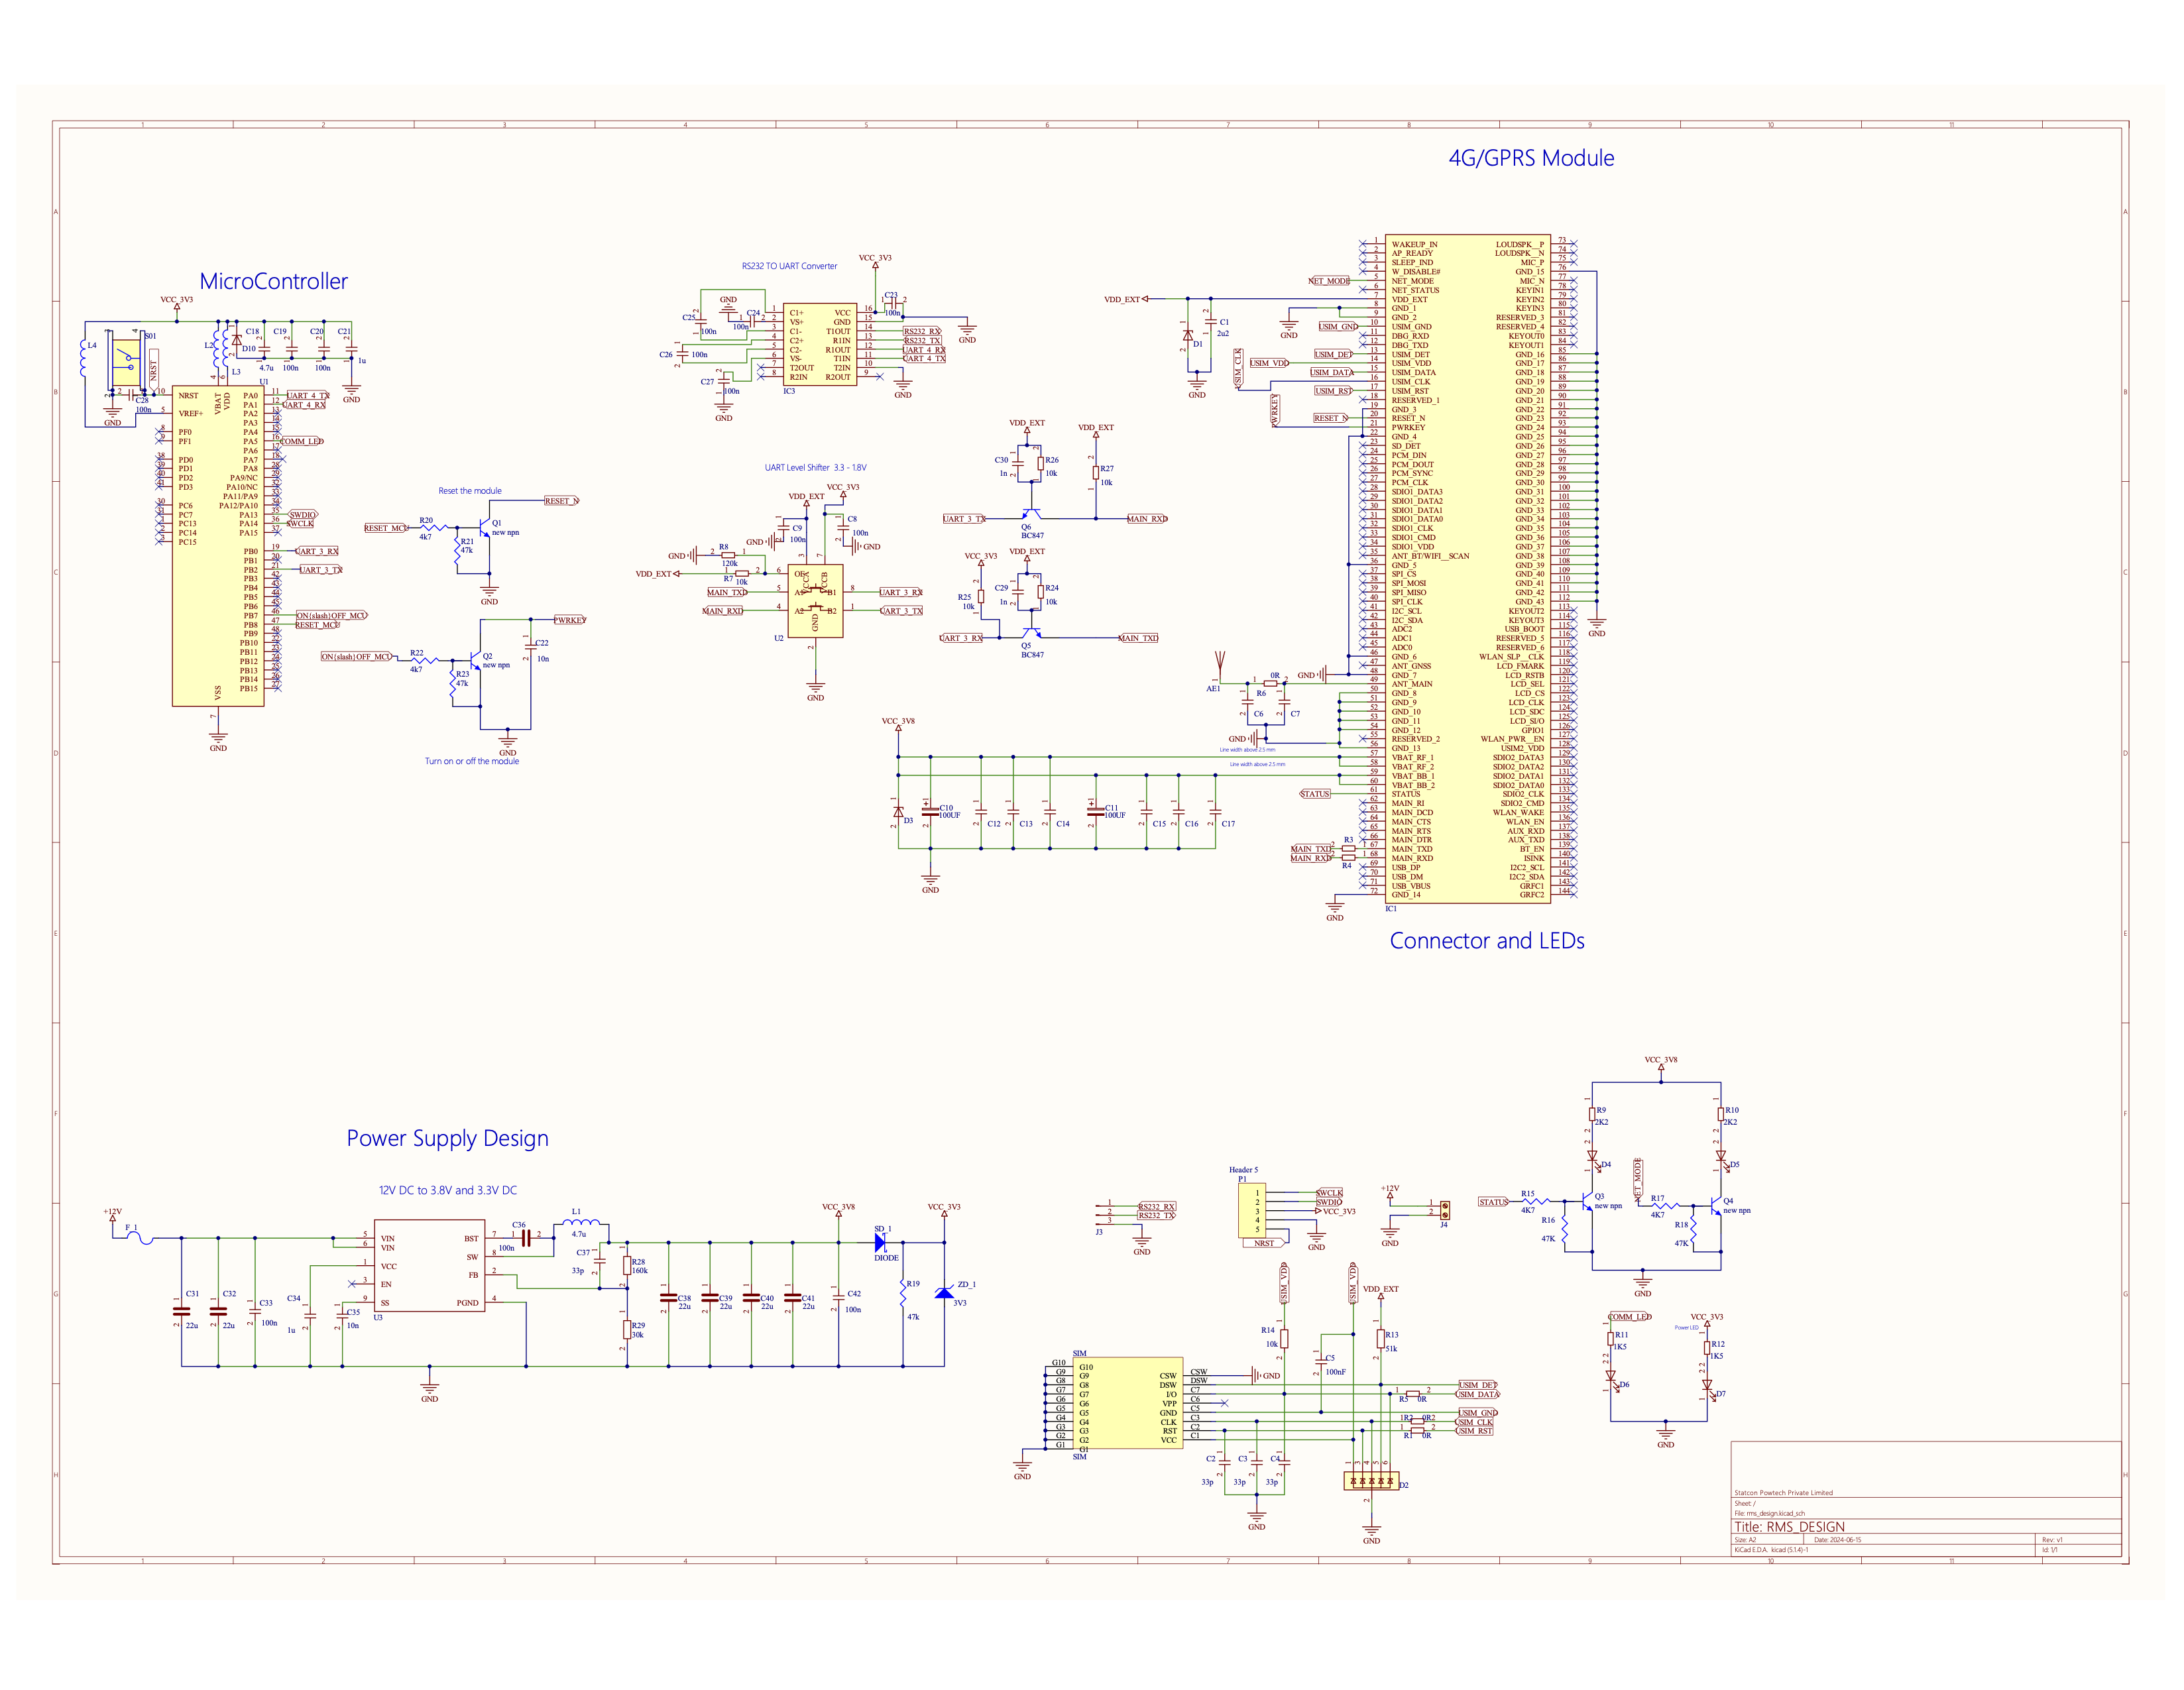
\includegraphics[width=0.85\textwidth]{images/schematic.png}
    \caption{Schematic of the Remote Monitoring System}
    \label{fig:schematic_rms}
\end{figure}
\begin{figure}[H]
    \centering
    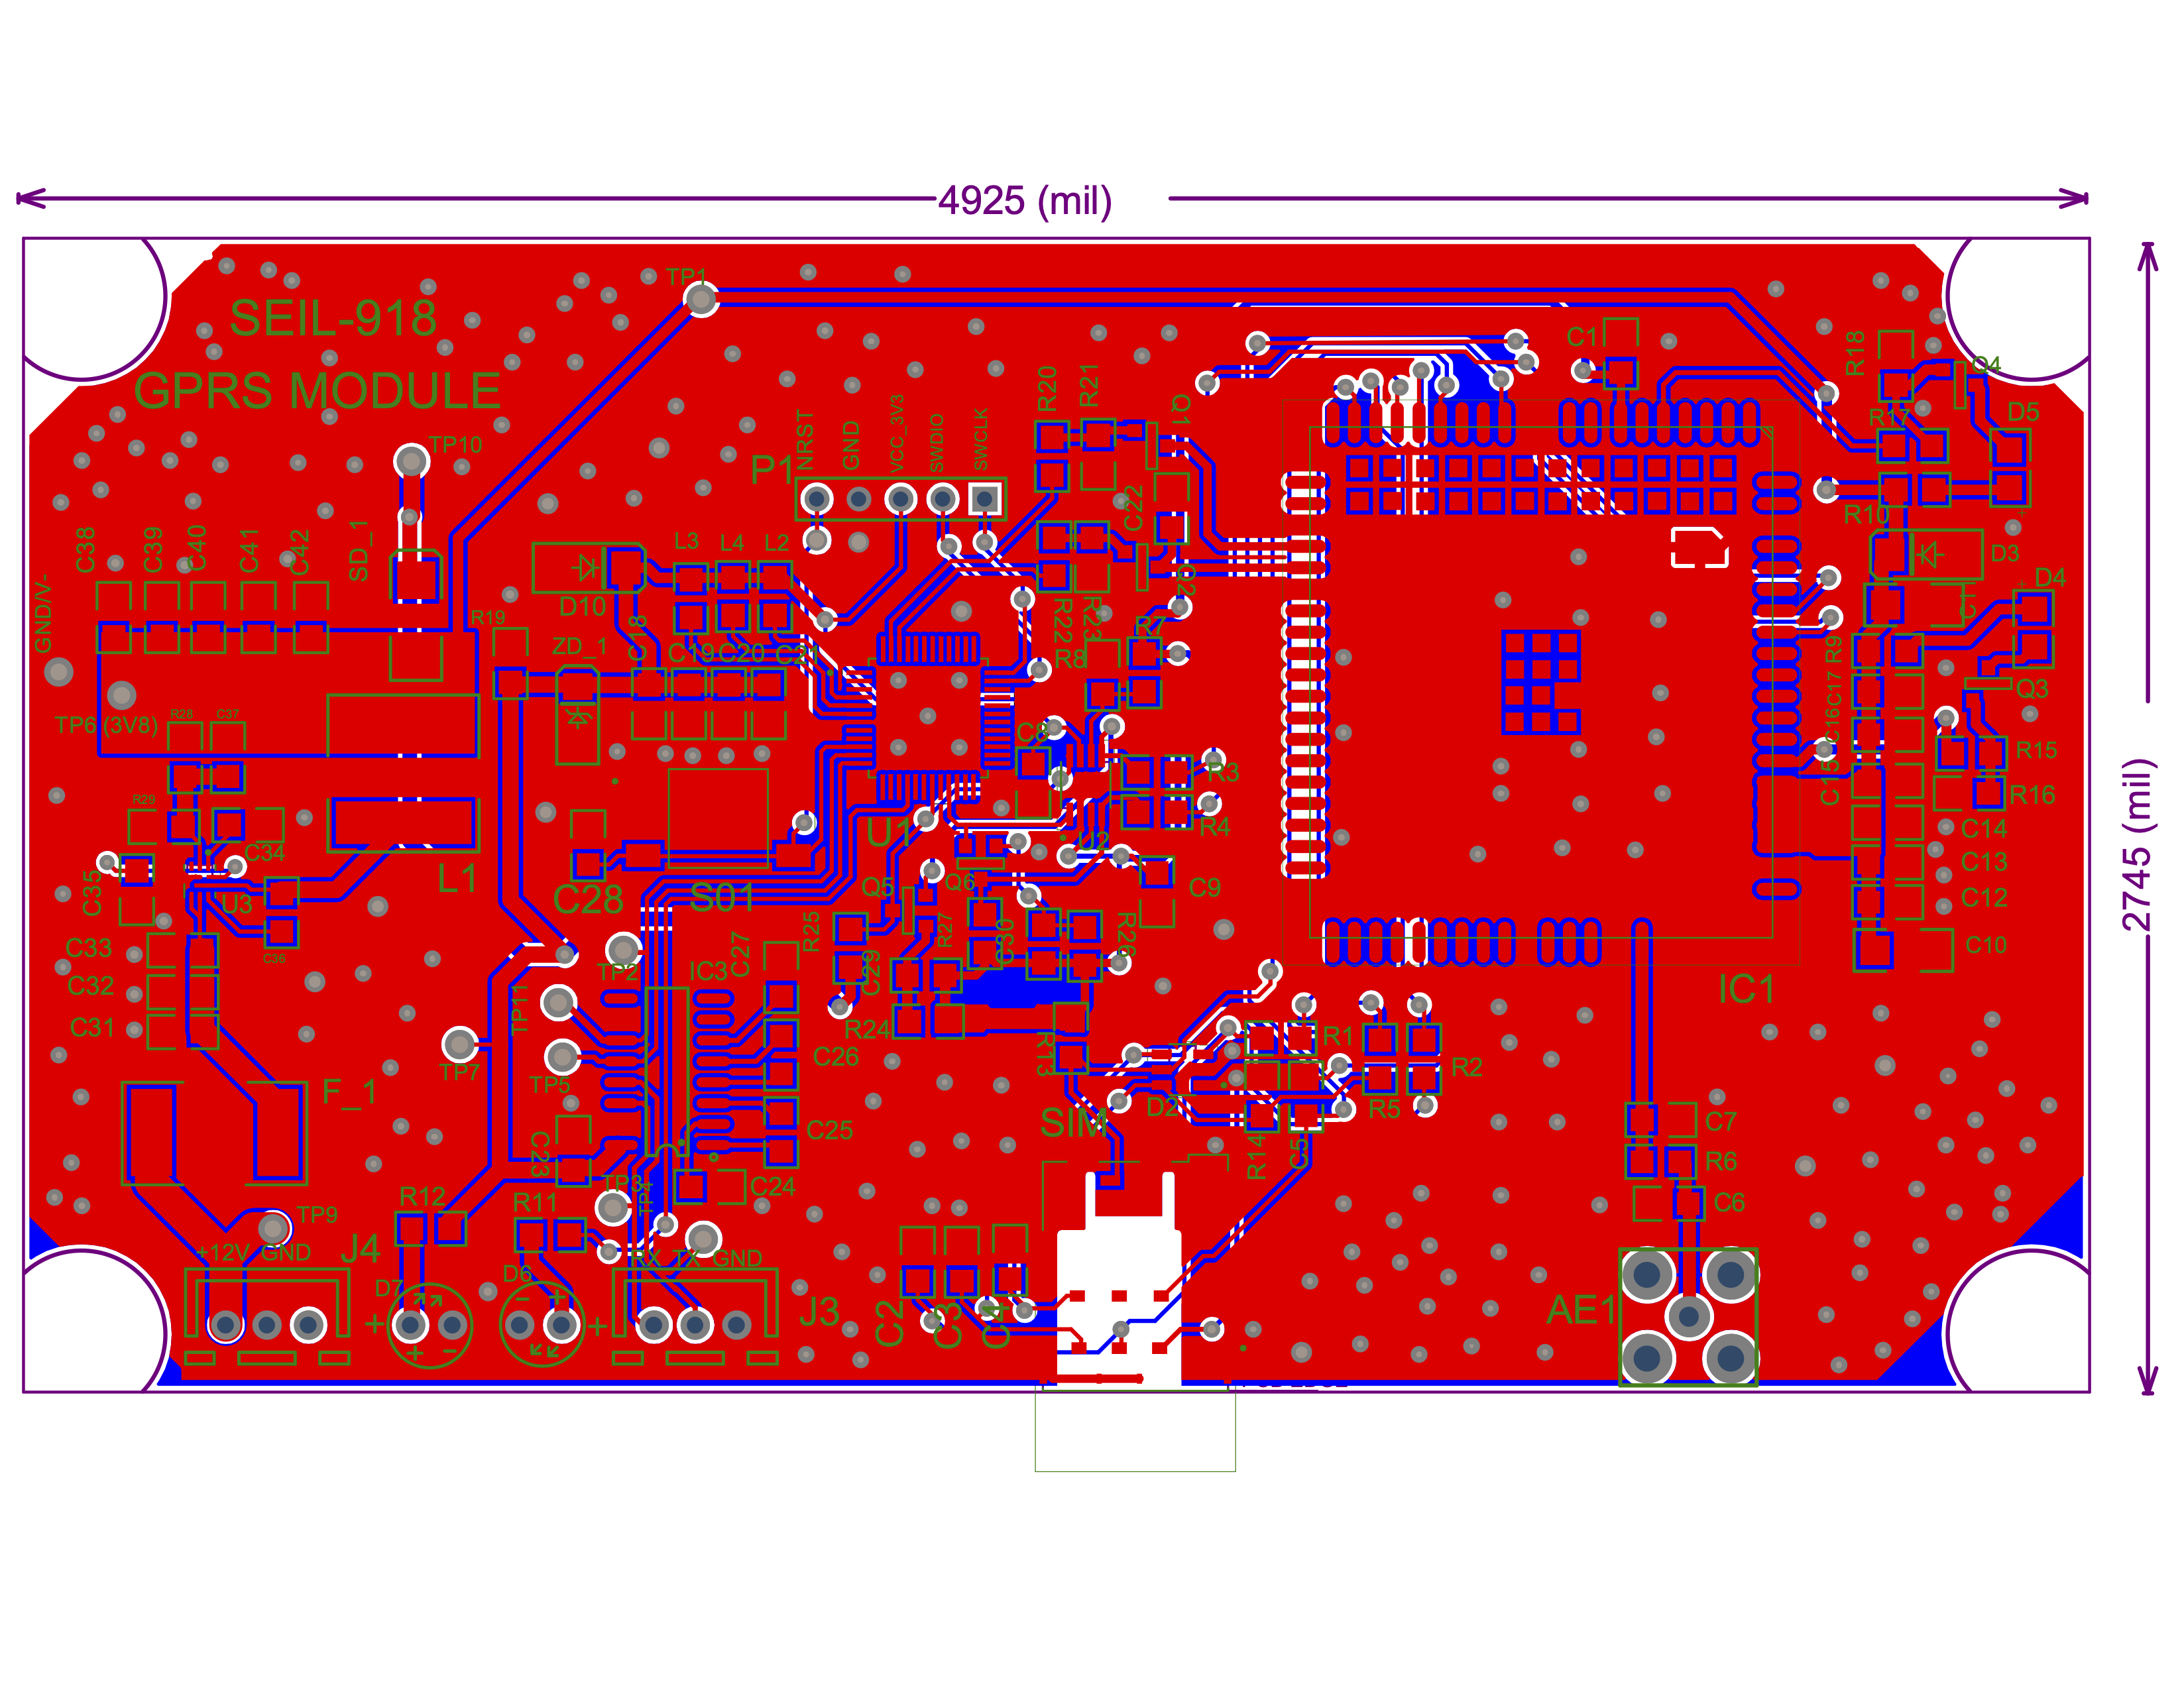
\includegraphics[width=0.85\textwidth]{images/pcb.png}
    \caption{PCB Layout of the Remote Monitoring System}
    \label{fig:pcb_rms}
\end{figure}